
The brain of human relies on oxygen which implies that the level of oxygen in air may influence mental performance. The density of oxygen is proportional to the density of air, which depends on pressure and temperature. After evaluating temperature and pressure as functions of altitude, we can conclude a formula describing air density.

Temperature at altitude $h$ meters above sea level can be approximated by the following formula (valid inside the troposphere):

$$T=T_0-Lh$$

\noindent where $T_0$ is the sea level standard temperature and $L$ is the temperature lapse rate.

The pressure at altitude $h$ is given by:

$$p = p_0 \left(1-\frac{Lh}{T_0}\right)^\frac{gM}{RL}$$

\noindent where $p_0$ is the sea level standard atmospheric pressure, $g$ is the earth-surface gravitational acceleration, $M$ is molar mass of dry air and $R$ is ideal gas constant.

According to the \emph{International Standard Atmosphere} the standard values are as follows:

\begin{align*}
T_0 &= \SI{288.15}{K}\\
L &= \SI{0.0065}{K/m}\\
p_0 &= \SI{101.325}{kPa}\\
g &= \SI{9.80665}{m/s^2}\\
M &= \SI{0.0289644}{kg/mol}\\
R &= \SI{8.31447}{J/(mol\cdot K)}
\end{align*}

Density can then be calculated using a molar form of the ideal gas law:

$$\rho = \frac{pM}{RT} = \frac{M p_0 \left(1-\frac{Lh}{T_0}\right)^\frac{gM}{RL}  }{ R (T_0-Lh)  }$$
\begin{figure}[ht]
	\centering
		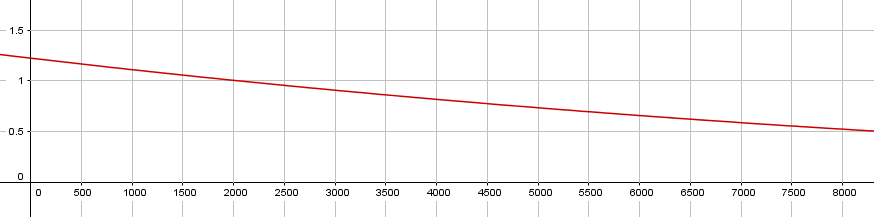
\includegraphics[width=\textwidth]{graph1}
    \caption{Air pressure based on altitude}
\end{figure}


Studies \cite{Scholey1999,Chung2008,Chung2004} confirm that increased amount of oxygen improves the cognitive performance of your mind. According to \cite{Chung2008}, hearth rate decreases with more concentrated oxygen in the air, as the blood cells carry more oxygen molecules. Following that, we can assume that lower air density, well known for causing a decrease in hearth rate, causes the opposite effect and lowers your mental performance.

Now we can use the results from various performance tests found in \cite{Research1996} to determine how cognitive function of a human is influenced by lower air pressure. The function that best fit the points of data from this research ended up being a logarithmic curve of the function:
\begin{center}
$f(x)=log_a\left(x-b\right)+c$
\end{center}
\begin{align*}
a &= 3.995\\
b &= 0.7576\\
c &= 14.05537
\end{align*}

\begin{figure}[ht]
	\centering
    	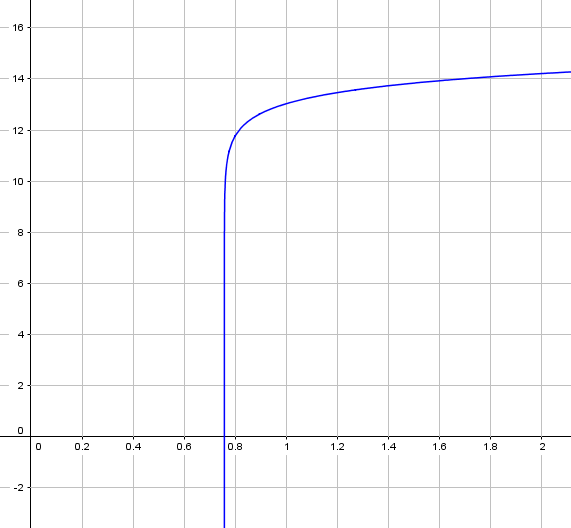
\includegraphics[width=0.4\textwidth]{graph2}
    \caption{Human productivity based on air pressure}
\end{figure}

Finally we need to combine both aforementioned functions:

$$g(h)=f(\rho)=log_a\left(\rho-b\right)+c=log_a\left(\dfrac{M p_0 \left(1-\dfrac{Lh}{T_0}\right)^{\dfrac{gM}{RL}}  }{ R (T_0-Lh)  }-b\right)+c$$

Using the variables mentioned before we can estimate a person's productivity in a certain altitude by dividing the value of $g(h)$ by the value of $g(0)$, in other word we will take a person's productivity at sea level as the base line. 

\begin{figure}[ht]
	\centering
    	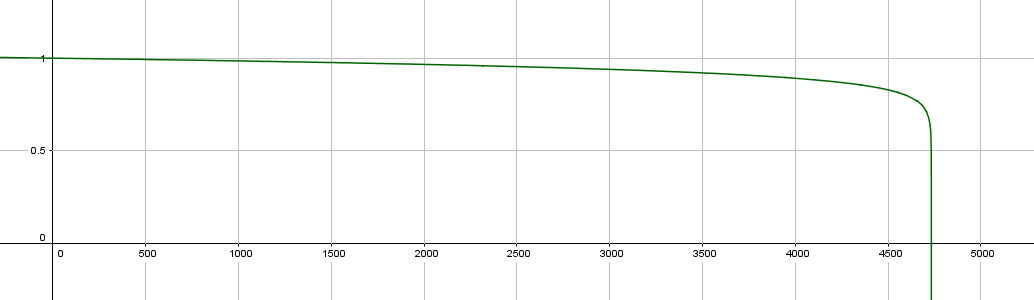
\includegraphics[width=\textwidth]{graph3}
    \caption{Human productivity based on altitude}
\end{figure}

$$ g(0) = log_a\left(\dfrac{M p_0 }{ R T_0  }-b\right)+c$$
$$P = \frac{g(h)}{g(0)} = \frac{ log_a\left(\dfrac{M p_0 \left(1-\dfrac{Lh}{T_0}\right)^{\dfrac{gM}{RL}}  }{ R (T_0-Lh)  }-b\right)+c }{ log_a\left(\dfrac{M p_0 }{ R T_0  }-b\right)+c }$$

A disadvantage of this approach is that because we used a logarithmic function to estimate the effect of air density on cognitive function our model behaves erratically for altitudes above $4600$ meters above sea level. In spite of that, we can safely use this model, because altitudes above $4600$ meters can be considered unsafe for an untrained person with no option of slow acclimatization and so such cases do not have to be examined.

When evaluating this factor, we will consider the effect on human performance on different days of the meeting to be equal. This position can be justified by the fact, that it may take considerably more time for a person with no previous experience of altitude acclimatization to get used to the new environment and even then the effects on a person's mental ability are likely to persist in some form. Our model may be further improved in this area by considering information from our attendees, about their previous high altitude experiences, however, currently not enough research has been done about these effects to create a more precise model.



